

\section{Experimental Results and Discussion}



Because we can either update pre-trained word embeddings during training or not, through the evaluation, we want to answer the following questions:
\begin{itemize}
\item How well do different word embeddings perform in all tasks when supervised fine-tuning is \textit{not} performed?
\item How well do different word embeddings perform in all tasks when supervised fine-tuning is performed?
\item How does the size of labeled training data affect the experimental results?
\item How well do the word embeddings perform for unknown words? 
\item How do the key parameters of each word learning algorithms affect the experimental results?
\end{itemize}

%%%%%%%%%%%%%%%%%%%%%%%%%%%%
%%% BESTS
\begin{figure*}
\caption{Best results for each method for POS-Tagging and Chunking}
\centering
\begin{subfigure}{.5\textwidth}
	\centering
    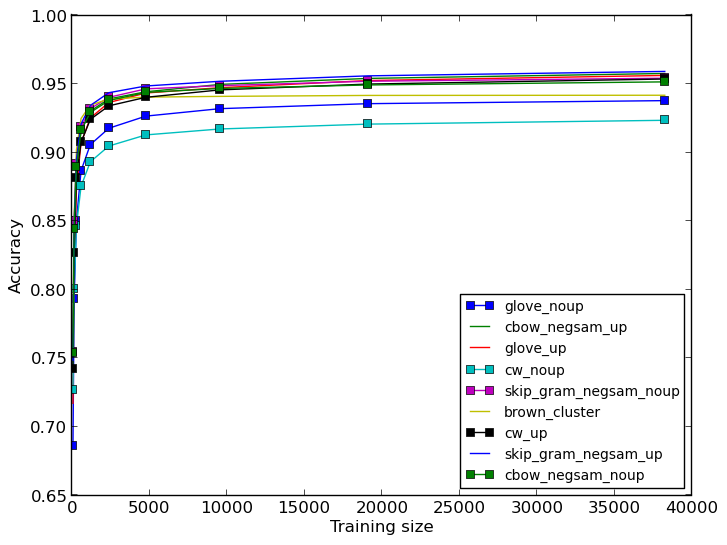
\includegraphics[width=0.8\textwidth]{plots/bestPOS.png}    	
	\label{fig:bestpos}
	\subcaption{POS-Tagging results}	
\end{subfigure}%
\begin{subfigure}{.5\textwidth}
	\centering
    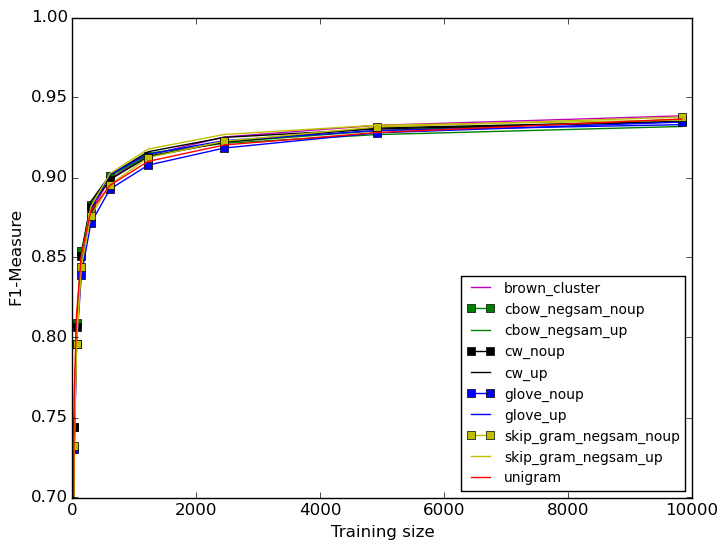
\includegraphics[width=0.8\textwidth]{plots/bestChunking.png}
	\label{fig:bestchunking}
	\subcaption{Chunking results}	
\end{subfigure}
\end{figure*}

\begin{figure*}
\caption{Best results for each method for NER and MWE}
\centering
\begin{subfigure}{.5\textwidth}
	\centering
    	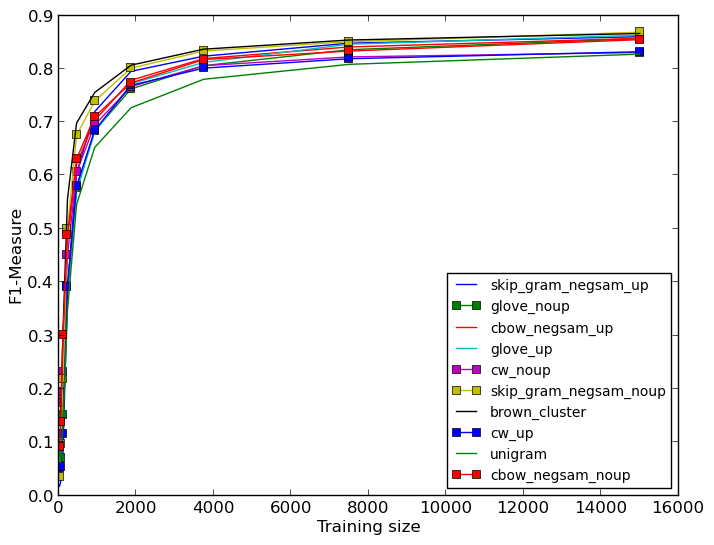
\includegraphics[width=0.8\textwidth]{plots/bestNER.png}
	\subcaption{NER results}	
	\label{fig:bestner}
\end{subfigure}
\begin{subfigure}{.5\textwidth}
	\centering
    	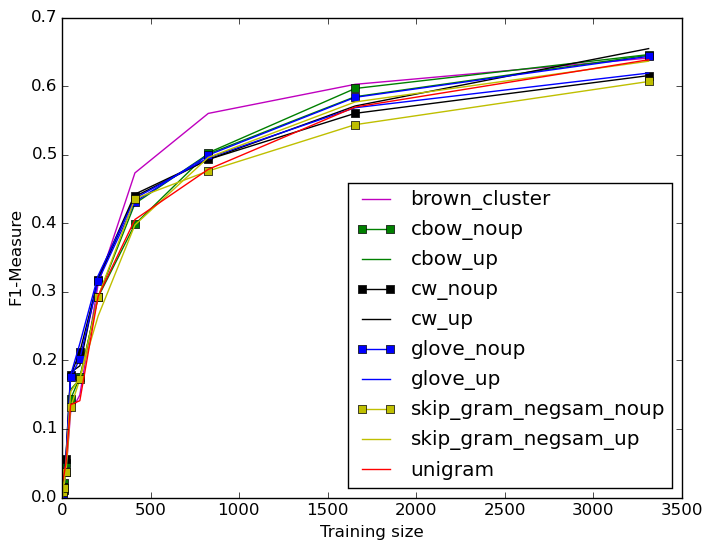
\includegraphics[width=0.8\textwidth]{plots/bestMWE.png}
    \subcaption{MWE results}	
	\label{fig:bestmwe}
\end{subfigure}  	
\end{figure*}  	


%%%%%%%%%%%%%%%%%%%%%%%%%%%%
%%% OUT OF VOC POS

\begin{figure*}
\caption{POS-Tagging out-of-vocabulary-words accuracy for \textit{in-domain} and \textit{out-of-domain} test sets}
\centering
\begin{subfigure}{.5\textwidth}
	\centering
    	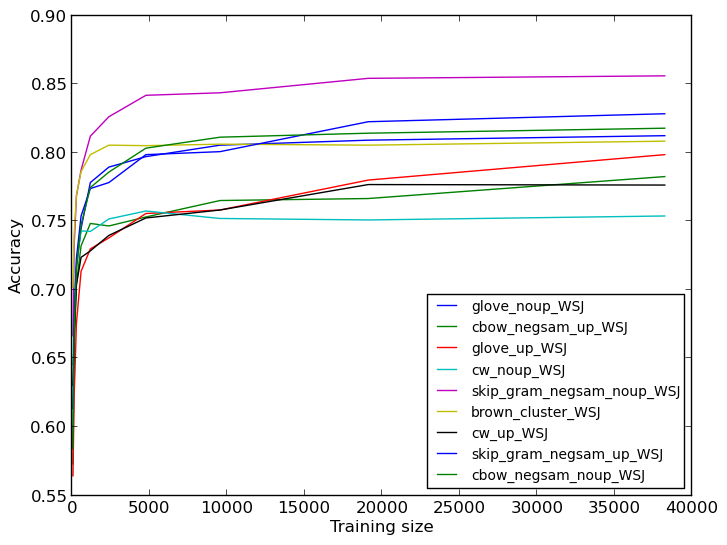
\includegraphics[width=0.8\textwidth]{plots/POSoutOfVocIN.png}
    	\subcaption{\textit{in domain} }
	\label{fig:inpos}
\end{subfigure}
\begin{subfigure}{.5\textwidth}
	\centering
    	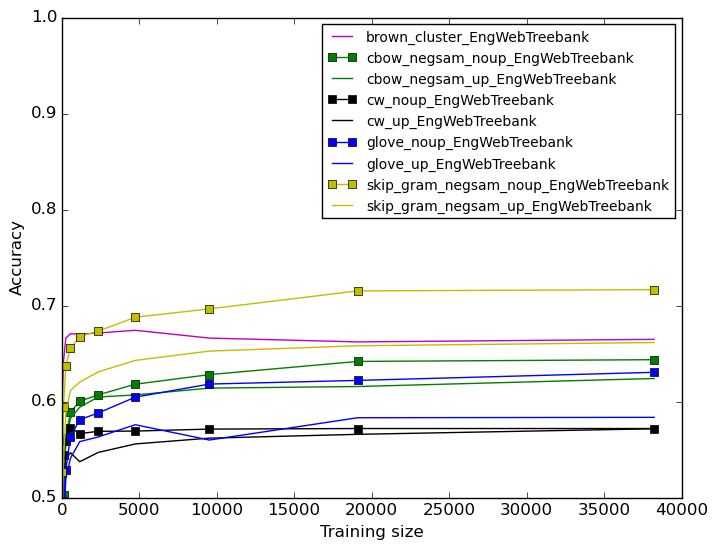
\includegraphics[width=0.8\textwidth]{plots/POSoutOfVocOUT.png}
   	\subcaption{\textit{out-of-domain}}
	\label{fig:outpos}
\end{subfigure}  	
\end{figure*} 

%%%%%%%%%%%%%%%%%%%%%%%%%%%%
%%% OUT OF VOC Chunking: missing result!!!

%%%%%%%%%%%%%%%%%%%%%%%%%%%%
%%% OUT OF VOC NER
\begin{figure*}
\caption{NER out-of-vocabulary-words accuracy for \textit{in-domain} and \textit{out-of-domain} test sets}
\centering
\begin{subfigure}{.5\textwidth}
	\centering
    	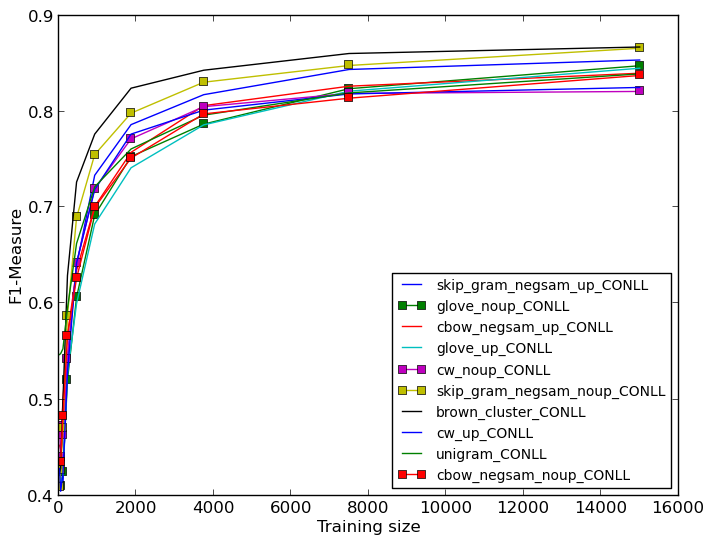
\includegraphics[width=0.8\textwidth]{plots/NERoutOfVocIN.png}
    	\subcaption{\textit{in-domain}}
	\label{fig:inner}
\end{subfigure}
\begin{subfigure}{.5\textwidth}
	\centering
    	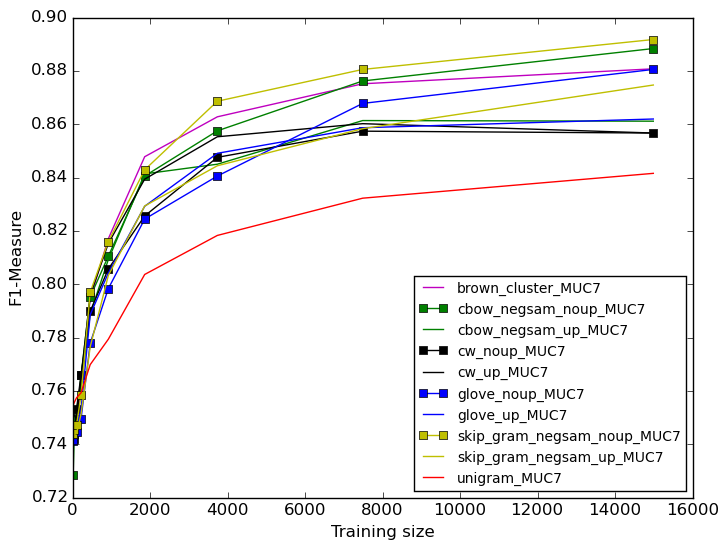
\includegraphics[width=0.8\textwidth]{plots/NERoutOfVocOUT.png}
   	\subcaption{\textit{out-of-domain}}
	\label{fig:outner}
\end{subfigure}  	
\end{figure*}


%%%%%%%%%%%%%%%%%%%%%%%%%%%%
%%% OUT OF VOC MWE
\begin{figure*}
\caption{MWE out-of-vocabulary-words accuracy for \textit{in-domain} test set}
\centering
    	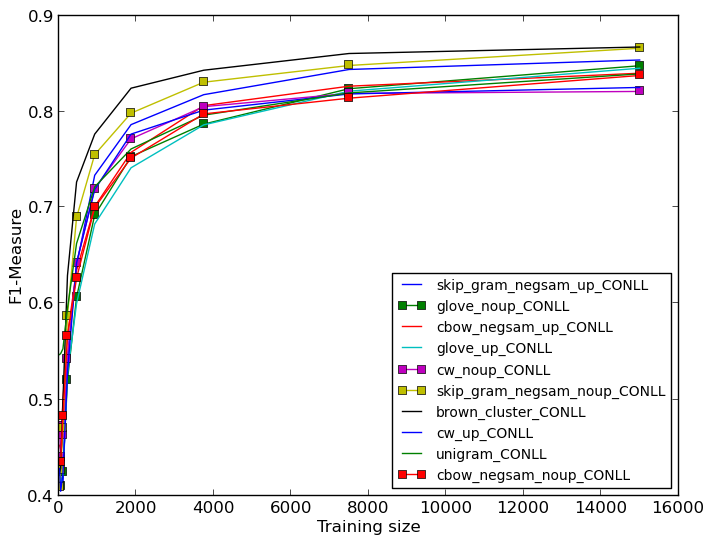
\includegraphics[width=0.5\textwidth]{plots/NERoutOfVocIN.png}    
\label{fig:outmwe}
\end{figure*}

%%%%%%%%%%%%%%%%%%%%%%%%%%%%
%%% OUT OF VOC POS




\section{Conclusion}
